\subsection{Logic Synthesis}
Having verified the correct functioning of the filter with Modelsim, Synopsys has been used for synthesis. The objective is to calculate the maximum frequency of operation of the circuit and then setting $T_{CLK} = 4 T_{min}$, compute the area and the dissipated power, using the data on switching activity produced by Modelsim.
The results related to the clock period, the associated slack and the area are shown in \autoref{tab:timing_rep_j}.

\begin{table}[h]
\begin{center}
\begin{tabular}{|l|l|l|}
\hline
$T_{CLK}$ (ns) & slack (ns) & area $(\SI{}{\micro\meter})^2$ \\
\hline
10 & 7.39 &  3200\\
0 & -1.75 &  3834\\
2.15 & 0 & 3542 \\
8.6 & 5.99 & 3200 \\
\hline
\end{tabular}
\end{center}
\caption{Results of timing report}
\label{tab:timing_rep_j}
\end{table}

Subsequently the net-list generated was used to determine the switching activity using Modelsim and obtain in this way an accurate estimation of the power consumption of the circuit. The results are shown in \autoref{fig:pow_rep_x4_j}.

\begin{figure}[h]
	\center
	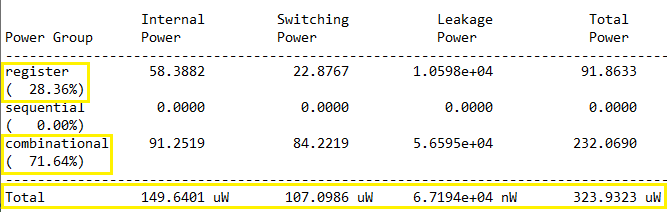
\includegraphics[width=0.8\textwidth]{report_power_x4_j_mod.png}
	\caption{Power Report}
	\label{fig:pow_rep_x4_j}
\end{figure}

Also in this case it is noted that the power consumption is mainly produced by the combinatorial part consisting of 3 adders and 4 multipliers.
Comparing the results of the two architectures implemented there are significant differences in terms of minimum period, in fact in the classic solution $T_{min}=\SI{4.10}{\nano\second}$, while in the J-look-ahead solution $T_{min}=\SI{2.15}{\nano\second}$, which corresponds to an increase in operating frequency of $48\%$. The performance enhancement is achieved thanks to the reduction of the critical path from 2 adders and 2 multipliers to only one multiplier. The improvement in performance, however, is paid for in terms of area, with an increase of $40\%$, and in terms of power. Comparing the data in \autoref{fig:pow_rep_x4} and \autoref{fig:pow_rep_x4_j} reveals an increase of $80\%$ in total power; specifically, the power contributions that change significantly are those related to the switching power, $\SI{2.3}{\micro\watt}$ versus $\SI{107.1}{\micro\watt}$, and to the internal power, $\SI{18.6}{\micro\watt}$ versus $\SI{149.6}{\micro\watt}$. The increase of these contributions is given by the fact that in the second architecture there are more logical blocks.

\subsection{Place \& Route}
The Place \& Route with the innovus software has been carried out following the previous procedure. The generated circuit is the one shown in \autoref{fig:layout_j}, it has an area equal to $\SI{3186}{\micro\meter}^2$ according to the one obtained from the Synopsys report, with a total of 1588 cells and 3993 gates. The values obtained are plausible if compared to those of the previous architecture because in this case there are more physical elements (registers, summers and multipliers) and consequently the need for more area to allocate all the necessary gates is expected.

\begin{figure}[h]
	\center
	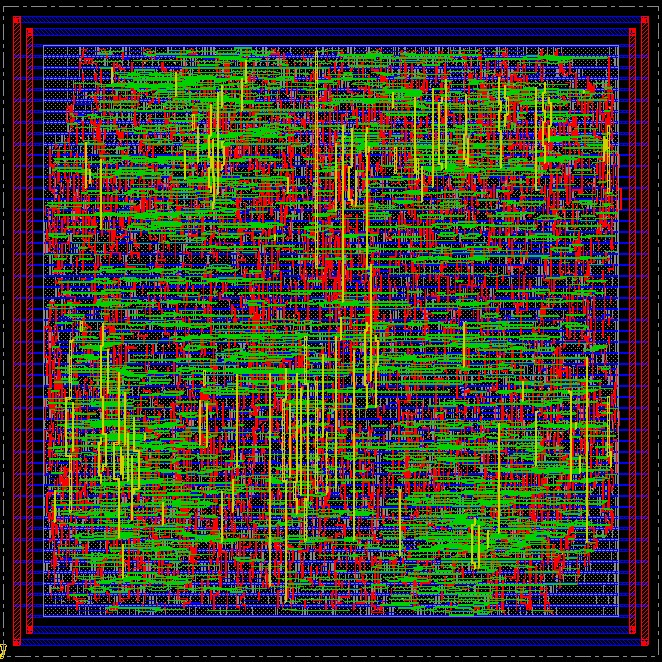
\includegraphics[width=0.6\textwidth]{IIR_filter_period_min_x4_place_j.jpg}
	\caption{Resulting layout}
	\label{fig:layout_j}
\end{figure}

Subsequently it was launched the timing analysis, the verification of connectivity and geometry, which showed the absence of any violation. Starting from the switching activity data obtained from Modelsim, an estimation of the power has been performed. The results are shown in \autoref{fig:cadence_pow_rep_x4_j}, also in this case the results obtained are in line with those obtained from the Synopsys power report.

\begin{figure}[h]
	\center
	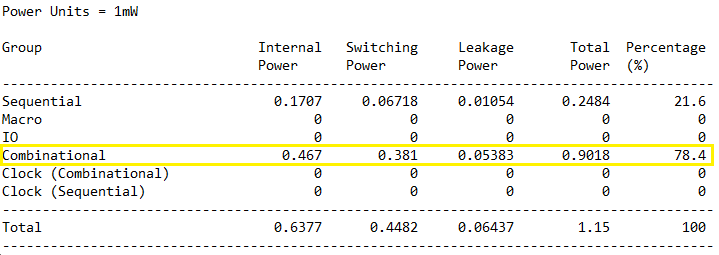
\includegraphics[width=0.8\textwidth]{rep_power_x4_cadence_j_mod.png}
	\caption{Post place \& route power report}
	\label{fig:cadence_pow_rep_x4_j}
\end{figure}